
\subsection{Completion, integrity and realized loss}\label{sec:completion}
The project completed the L12/H1 primary setting, six secondary settings and the external frozen-weight transfer. It retained 364 final neural fits and 56 simple model/setting/resource records, with 280 short source-only candidate fits. The complete new study contains 9680 saved prediction arrays and 3,097,600 service-level metric rows. An independent float64 reconstruction from all arrays checked target indices and counts, array digests, MAE, RMSE and MASE against the saved CSVs. The largest absolute metric reconstruction difference was $3.73\times10^{-9}$ in physical units. The 420 final checkpoints and frozen-source hashes passed the checkpoint audit. These rows are repeated model/seed/mask/condition/service summaries, not independent data sources.

At nominal 20\% loss, the four exact-count mechanisms produced 19.988\% induced unavailability on the ChronoGraph test segment; lag-MAR averaged 26.301\% across twenty masks, ranging from 25.925\% to 26.577\%. In the 48-bin external case, rounding gives 20.833\% for exact-count mechanisms, while lag-MAR averaged 27.861\% (26.042\%--30.469\%). Natural missingness is recorded separately. Fig.~\ref{fig:masks} makes the imposed spatial and duration structure visible. The 70/10/20 source cut is a row split; the external case has 12 calibration and 36 target bins.

\subsection{Primary 32-service comparison}
Table~\ref{tab:primary} and Fig.~\ref{fig:models} report the prespecified six positive-loss original conditions at L12/H1. PatchTST has the lowest observed mean MASE, 1.0419 for CPU and 1.2170 for memory; NLinear is close at 1.0463 and 1.2197. No confirmatory comparison between those two models was specified. Moving average has CPU MASE1.0678, below DLinear (1.1493), E5 (1.1454) and A3 (1.1602). For memory, A0 is the lowest compact affine variant at 1.2334, whereas A3 is 1.2403, DLinear 1.2402 and E5 1.2656. Thus the two added availability coefficients do not produce an aggregate A3 gain over A0. E5's favorable historical memory result does not carry over as a win over DLinear in this new cohort. The graph GRU's memory MASE is 1.4851; none of the neural families was removed because of an unfavorable score.

\begin{table*}[!t]
\caption{Primary new-service means over equal service, original positive-loss condition, mask and seeded-fit weights. CPU absolute MAE/RMSE are displayed in $10^{-3}$ publisher-scale units; memory absolute errors are in MiB ($2^{20}$ bytes). MASE is dimensionless. Lower is better. No significance is inferred from rank alone.}\label{tab:primary}
\centering\footnotesize
\FitTable{\begin{tabular}{lrrrrrr}
\toprule
Model & CPU MASE & CPU MAE & CPU RMSE & Mem. MASE & Mem. MAE & Mem. RMSE \\
\midrule
Persistence & 1.1170 & 3.3236 & 4.5878 & 1.2861 & 2.0009 & 3.3833 \\
Moving average & 1.0678 & 2.9643 & 4.2038 & 1.2361 & 1.8956 & 3.2699 \\
Exponential smoothing & 1.0691 & 2.8926 & 4.0646 & 1.2535 & 1.9130 & 3.2673 \\
Ridge & 1.2669 & 3.1952 & 4.3079 & 1.3613 & 1.9589 & 3.1848 \\
DLinear & 1.1493 & 2.9924 & 4.1015 & 1.2402 & 1.8762 & 3.1573 \\
NLinear & 1.0463 & 2.8499 & 3.9969 & 1.2197 & 1.8482 & 3.1422 \\
E5 & 1.1454 & 3.0142 & 4.1411 & 1.2656 & 1.9044 & 3.1560 \\
A0 & 1.1562 & 3.0028 & 4.1185 & 1.2334 & 1.8649 & 3.1605 \\
A1 & 1.1547 & 2.9986 & 4.1147 & 1.2397 & 1.8704 & 3.1591 \\
A2 & 1.1563 & 3.0030 & 4.1185 & 1.2443 & 1.8773 & 3.1650 \\
A3 & 1.1602 & 3.0095 & 4.1248 & 1.2403 & 1.8733 & 3.1629 \\
GRU (own) & 1.2198 & 3.2253 & 4.5667 & 1.3438 & 2.1652 & 3.7094 \\
GRU (graph) & 1.1949 & 3.2375 & 4.5153 & 1.4851 & 2.2017 & 3.6563 \\
GRU-D adaptation & 1.1766 & 3.1392 & 4.4427 & 1.3605 & 2.1647 & 3.6811 \\
PatchTST (small) & 1.0419 & 2.8539 & 4.1061 & 1.2170 & 1.8649 & 3.1655 \\
\bottomrule
\end{tabular}
}
\end{table*}

\begin{figure*}[!t]\centering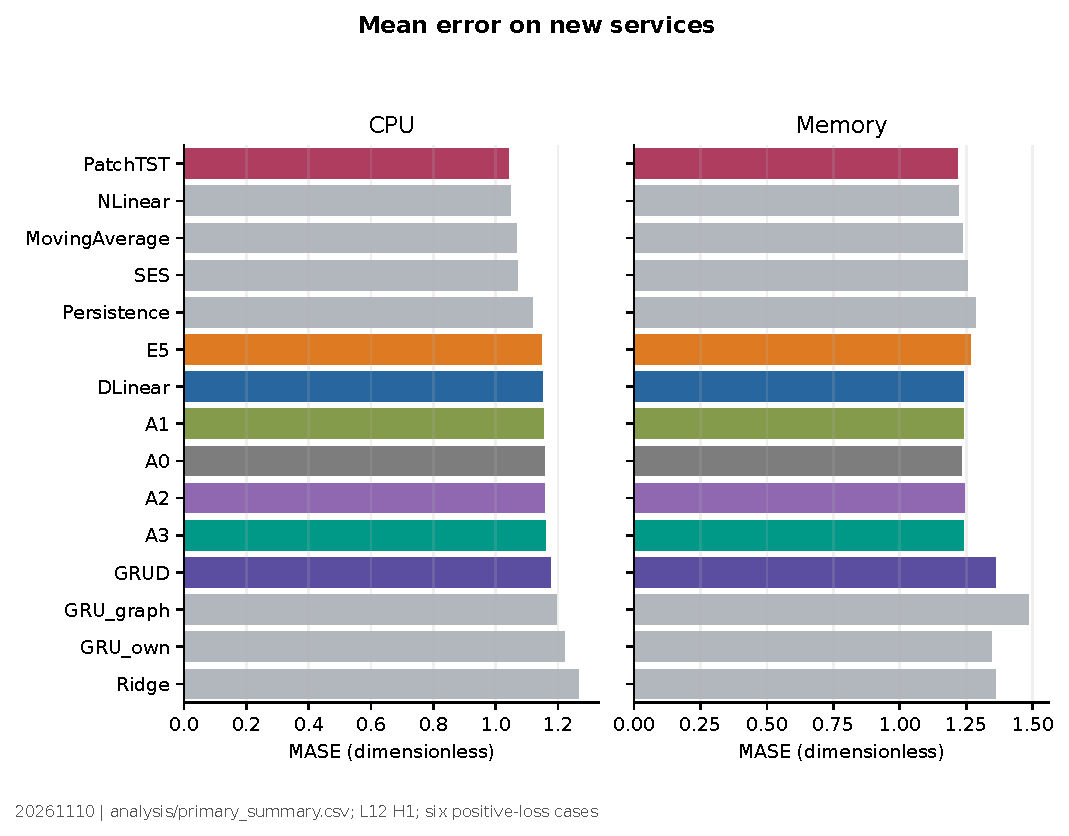
\includegraphics[width=0.79\textwidth]{figuras/06_models.pdf}
\caption{Primary MASE for all 15 newly evaluated families. CPU ordering is only a display choice. Families share the same fixed services, masks and target origins, while neural seed variability remains visible in supplementary material.}\label{fig:models}\end{figure*}


\subsection{Four prespecified paired contrasts}\label{sec:contrasts}
Table~\ref{tab:contrasts} distinguishes a mean MASE difference from a mean per-cell percentage reduction. The sole contrast with ten of ten favorable seed means is A3 versus E5 on memory: $\Delta=0.02523$ MASE, Holm-adjusted exact sign-test $p=0.0078125$, and a conditional 48-step crossed-block 95\% interval $[0.01312,0.03981]$. The mean paired per-cell reduction is 1.00\%; the ratio of aggregate means gives 1.99\%, a different estimand. Excluding the source-tuning seed 101 leaves nine of nine favorable seed means and an exploratory separately adjusted $p=0.015625$. These values concern fixed services, masks and trace and do not establish improvement in a population of cloud systems.

A3 versus DLinear has negative mean $\Delta$ on CPU ($-0.01090$) and nearly zero on memory ($-0.00014$); the adjusted sign-test $p$ is 1 for both. A3 versus E5 on CPU is also negative ($-0.01485$, adjusted $p=1$). Its conditional temporal bootstrap interval excludes zero on the negative side, whereas only three of ten seed means favor A3 and the prespecified sign test is nonsignificant. The two procedures address different sampling assumptions and estimands; the interval does not override the four-test decision rule. Primary block-length sensitivity is listed in Table~\ref{tab:block}.

\begin{table*}[!t]
\caption{Four prespecified A3 contrasts. $\Delta$MASE is reference minus A3; positive values favor A3. Mean $R$ averages paired valid cell percentages, rather than taking a ratio of overall means. Intervals resample seed, mask and time blocks conditional on fixed services; $p$ values are exact two-sided seed-mean sign tests adjusted by Holm.}\label{tab:contrasts}
\centering\footnotesize
\FitTable{\begin{tabular}{lrrrrrr}
\toprule
Resource & Reference & $\Delta$MASE & Mean $R$ (\%) & Conditional 95\% interval & $p_{\mathrm{Holm}}$ & Positive seeds \\
\midrule
CPU & DLinear & -0.01090 & -0.78 & [-0.02732, 0.00470] & 1 & 4/10 \\
CPU & E5 & -0.01485 & -1.95 & [-0.02977, -0.00120] & 1 & 3/10 \\
Memory & DLinear & -0.00014 & 0.00 & [-0.00959, 0.01035] & 1 & 3/10 \\
Memory & E5 & 0.02523 & 1.00 & [0.01312, 0.03981] & 0.007812 & 10/10 \\
\bottomrule
\end{tabular}
}
\end{table*}

The favorable memory mean against E5 is spatially uneven: only 10 of 32 service-level paired mean differences favor A3. Service540 alone contributes 42.4\% of the aggregate mean difference. An outcome-informed \emph{post hoc} sensitivity excluding it still yields a positive mean difference of 0.01499; excluding the three largest favorable services yields 0.00325 and six of ten favorable seed means. These exclusions were chosen after seeing outcomes, so neither resulting sign-test value is confirmatory. Fig.~\ref{fig:services} displays the separately specified DLinear--A3 service differences, which are also heterogeneous. Table~\ref{tab:variation} separates seed and mask variation. Fig.~\ref{fig:seeds} shows the between-fit spread, while Fig.~\ref{fig:ablation} shows that adding both descriptors does not guarantee lower mean error. Masks repeat the evaluation of the same fits.

\begin{figure*}[!t]\centering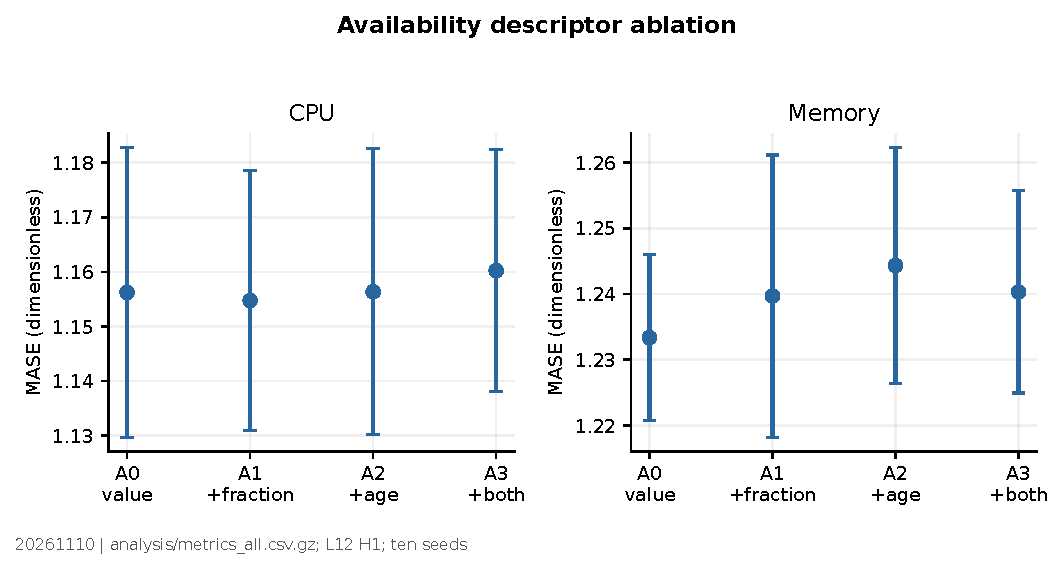
\includegraphics[width=0.79\textwidth]{figuras/11_ablations.pdf}
\caption{A0--A3 means and standard deviations across ten seeded-fit means. Error bars are descriptive standard deviations, not confidence or prediction intervals. Each family was independently tuned on source validation.}\label{fig:ablation}\end{figure*}
\begin{figure*}[!t]\centering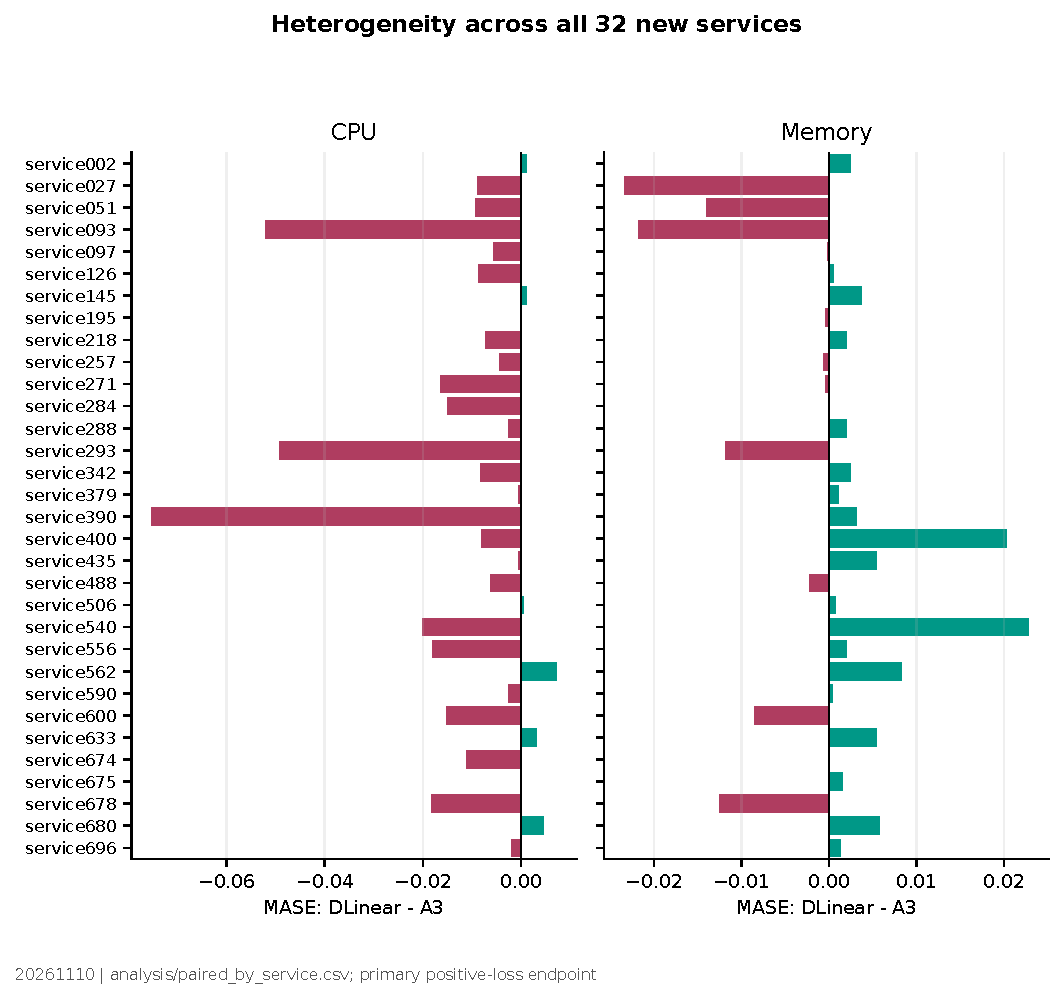
\includegraphics[width=0.71\textwidth]{figuras/15_services.pdf}
\caption{DLinear minus A3 MASE by destination service, averaged over paired seeds, masks and six positive-loss conditions. Positive bars favor A3. These connected services are fixed study cases rather than independent population draws.}\label{fig:services}\end{figure*}

\begin{figure*}[!t]\centering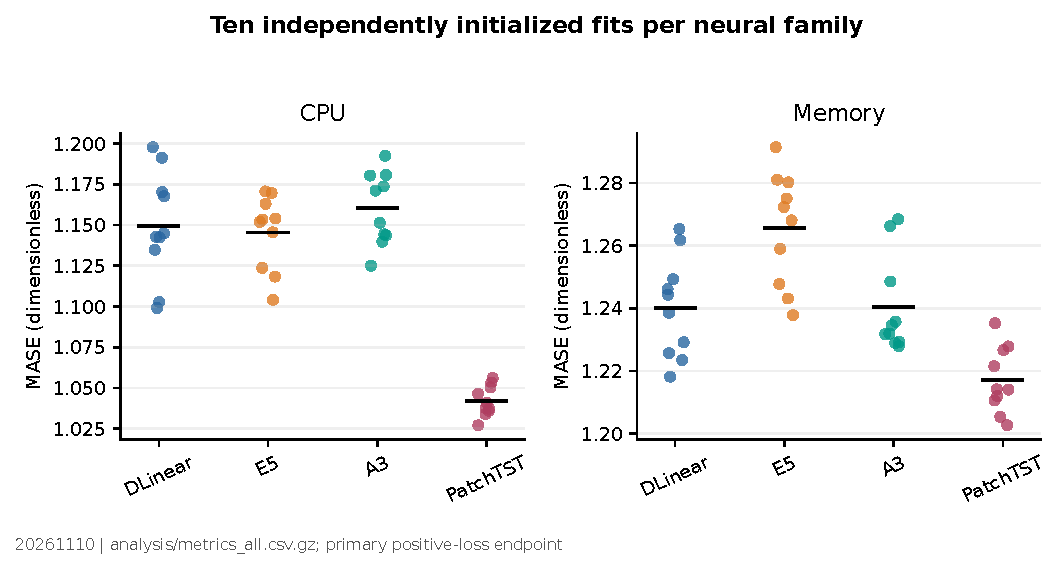
\includegraphics[width=0.76\textwidth]{figuras/10_seed_variability.pdf}
\caption{Ten seeded fit means per displayed neural family, averaged over fixed services, six positive-loss conditions and twenty masks. Black marks denote their mean. These are initialization replicates, not ten infrastructures.}\label{fig:seeds}\end{figure*}
\subsection{Robustness to incomplete telemetry}
Mean error generally rises from complete telemetry to 40\% missingness in the displayed scattered and short-block curves (Fig.~\ref{fig:loss}). This describes model averages, not a monotonicity theorem for every service or mask. At nominal 20\%, prolonged blocks are harder than correlated masks for A3: CPU MASE1.2330 versus 1.1342 and memory 1.3743 versus 1.1932. Lag-MAR is not directly a controlled 20\% comparison because its realized missing fraction is higher. Table~\ref{tab:stress} retains all models and all three added mechanisms; no claim is based on selecting favorable curves alone.

\begin{figure*}[!t]\centering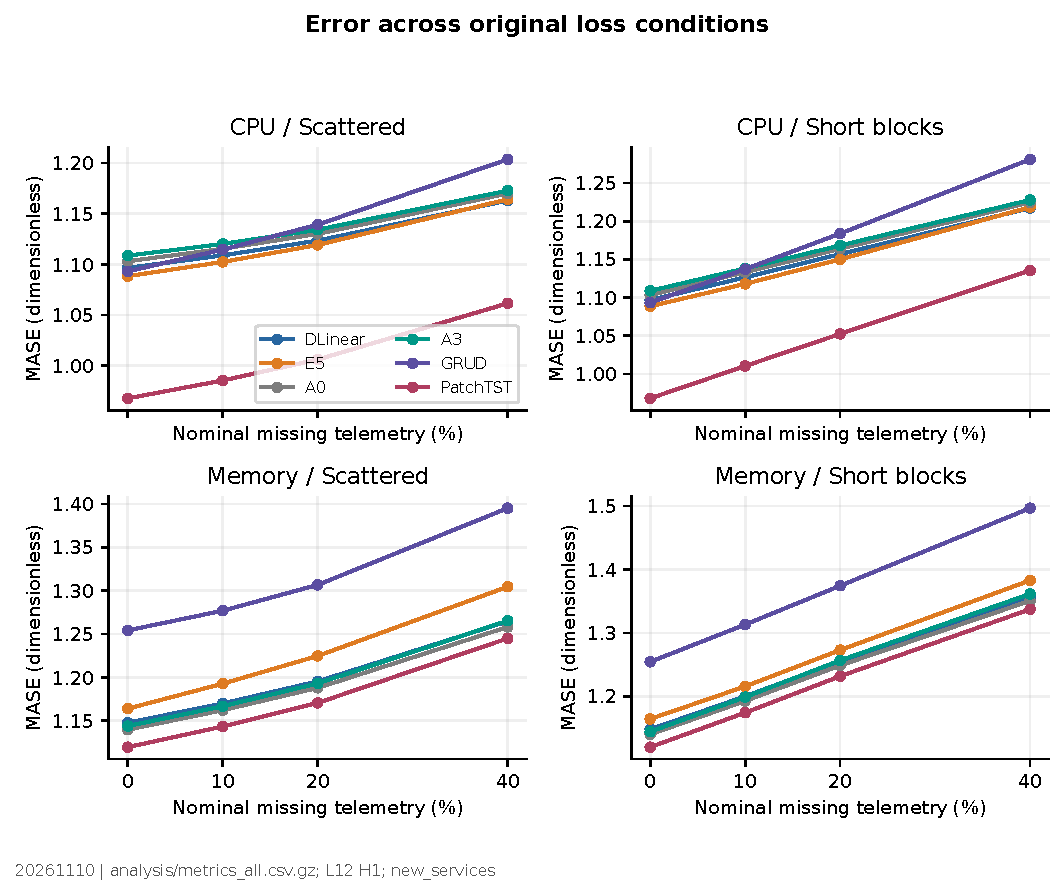
\includegraphics[width=0.76\textwidth]{figuras/07_loss.pdf}
\caption{Descriptive mean MASE under the original complete, scattered and short-block conditions. The six curves shown were chosen for display; Table~\ref{tab:primary} and machine-readable CSVs retain the complete comparison.}\label{fig:loss}\end{figure*}
\subsection{Direct horizons and input histories}
The common-support secondary display uses 1553 identical destination target rows (6452--8004), the first three training seeds, five paired masks and the original six positive-loss conditions. With L12, PatchTST's observed CPU MASE increases from 1.0445 at 30 minutes to 1.6399 at six hours; A3 increases from 1.1584 to 1.9779. Memory increases from 1.2264 to 2.1681 for PatchTST and from 1.2436 to 2.3141 for A3. Each horizon has a separately fitted direct model; these are not iterated one-step predictions. Longer histories at 30 minutes are mixed: A3 CPU improves from 1.1584 (L12) to 1.0966 (L48), while its memory MASE rises from 1.2436 to 1.2560. PatchTST memory is lowest at L24 (1.2190) among its three displayed history lengths. The common-support H30 point deliberately differs from the full primary endpoint and is not a replacement test. Figs.~\ref{fig:horizon} and~\ref{fig:history} and Tables~\ref{tab:horizon}--\ref{tab:history} retain the star-design comparisons.
\begin{figure*}[!t]\centering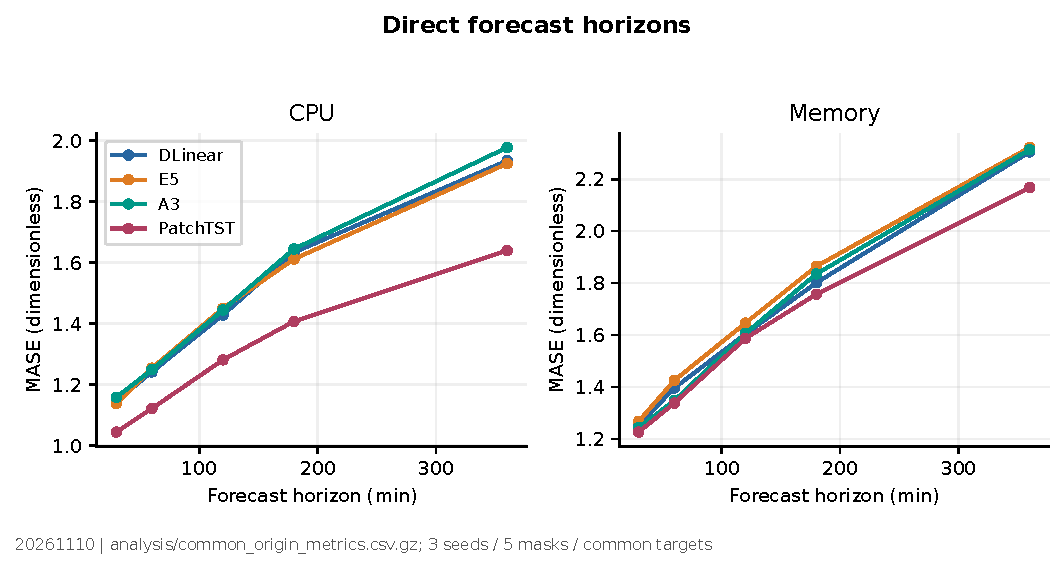
\includegraphics[width=0.79\textwidth]{figuras/08_horizon.pdf}
\caption{Common-target-origin direct-horizon MASE, three seeds and five masks. Each endpoint is fitted directly, using the same fixed 1553 target rows for display; no complete factorial is implied.}\label{fig:horizon}\end{figure*}
\begin{figure*}[!t]\centering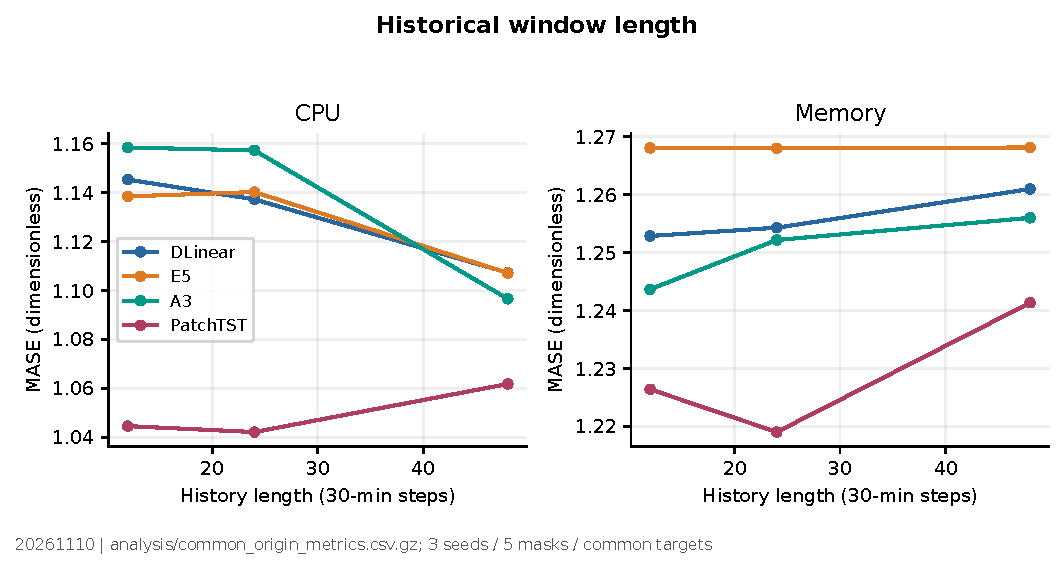
\includegraphics[width=0.79\textwidth]{figuras/09_history.pdf}
\caption{Common-target-origin history sensitivity at a 30-minute horizon, with the same three-seed/five-mask subset. Lines are descriptive and have no confirmatory significance tests.}\label{fig:history}\end{figure*}

\subsection{External transfer and computational cost}\label{sec:cost}
Fig.~\ref{fig:external} shows the external ranking. In the Alibaba day, persistence gives the lowest observed MASE of the 14 eligible families for both normalized CPU (2.3795) and normalized memory (7.5150). A3 is 3.3593 and 9.9535; PatchTST is 3.1112 and 10.5876. No method is retuned on these 36 target bins, and graph GRU is absent because its external graph is unavailable. The short six-hour MASE denominator and target-aggregation differences constrain interpretation. Absolute errors in Table~\ref{tab:external} are normalized utilization, not comparable with ChronoGraph bytes or CPU scale. The rankings contradict any universal transfer advantage from the primary setting.
\begin{figure*}[!t]\centering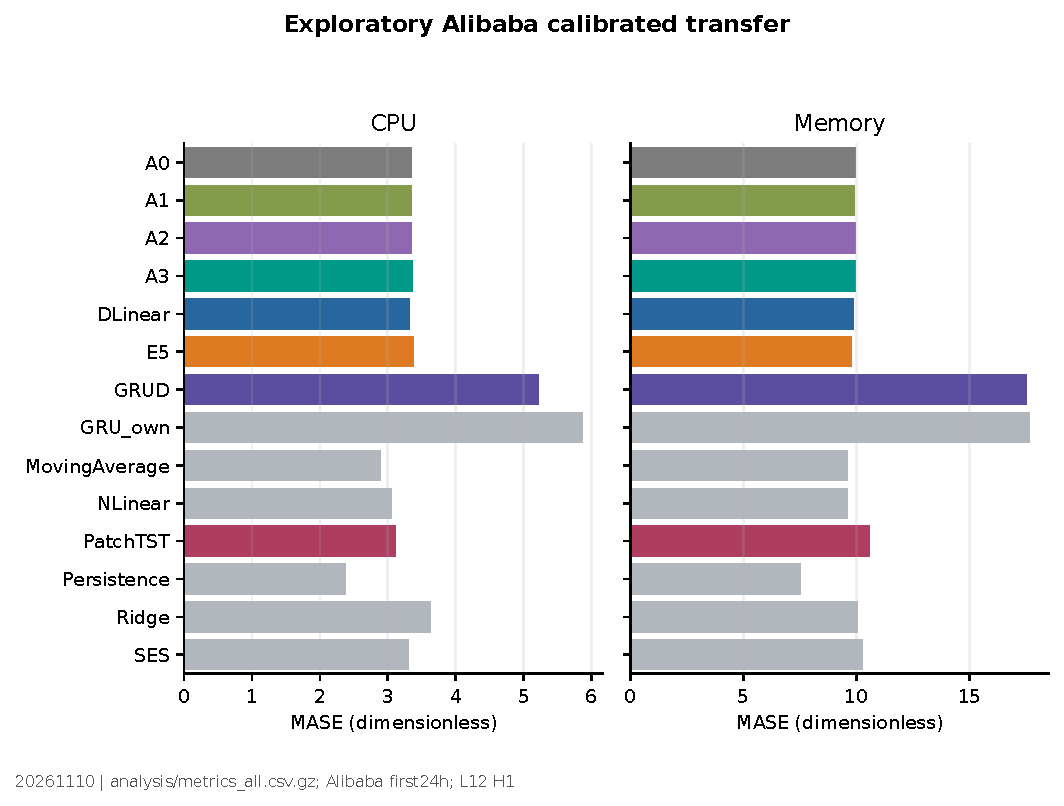
\includegraphics[width=0.79\textwidth]{figuras/12_external.pdf}
\caption{Exploratory first-day Alibaba transfer. Bars show MASE on 32 availability-selected services and 36 half-hour targets after a six-hour calibration prefix. These bars do not represent independent-infrastructure validation.}\label{fig:external}\end{figure*}

At L12, A3 uses 15 trainable parameters per resource versus DLinear's 26 and E5's 74. For a batch of one origin with 32 services, measured CPU p50 forward latency is 0.050 ms for A3, 0.057 ms for DLinear and 0.295 ms for E5; synchronized CUDA p50 is 0.141, 0.281 and 0.665 ms, respectively. PatchTST has 2499 trainable elements, CPU p50 0.521 ms and CUDA p50 1.212 ms. These samples show an observed accuracy/cost tradeoff under resident-input inference, not total monitoring latency or a causal hardware-wide speedup. On this small batch, CUDA is slower than CPU for some compact references. Completed-epoch time medians, including validation, are 8.56 s for A3, 10.21 s for DLinear, 14.72 s for E5 and 42.88 s for PatchTST; these exclude tuning, checkpoint I/O and failed incomplete attempts. Table~\ref{tab:efficiency} includes p95 values and all families. Fig.~\ref{fig:latency} relates the measured forward times to CPU error, and Fig.~\ref{fig:params} shows that a similar size can accompany different MASE values.
\begin{table*}[!t]
\caption{Trainable elements and measured p50/p95 forward latency in ms at B1/32 services. CUDA rows synchronize each trial; GRU-D CUDA uses replay without capture setup. Epoch sum is the median completed source-fit epoch-time sum over primary seeded fits, not total research time.}\label{tab:efficiency}
\centering\footnotesize
\FitTable{\begin{tabular}{lrrrrrr}
\toprule
Model & Parameters & CPU p50 & CPU p95 & CUDA p50 & CUDA p95 & Epoch sum (s) \\
\midrule
Persistence & 0 & 0.005 & 0.005 & 0.012 & 0.012 & not timed \\
Moving average & 0 & 0.014 & 0.015 & 0.023 & 0.025 & not timed \\
Exponential smoothing & 0 & 0.195 & 0.417 & 0.328 & 0.337 & not timed \\
Ridge & 13 & 0.022 & 0.024 & 0.084 & 0.092 & not timed \\
DLinear & 26 & 0.057 & 0.064 & 0.281 & 0.337 & 10.21 \\
NLinear & 13 & 0.031 & 0.045 & 0.095 & 0.102 & 7.62 \\
E5 & 74 & 0.295 & 0.317 & 0.665 & 0.681 & 14.72 \\
A0 & 13 & 0.022 & 0.023 & 0.085 & 0.095 & 7.26 \\
A1 & 14 & 0.046 & 0.049 & 0.125 & 0.134 & 7.99 \\
A2 & 14 & 0.030 & 0.032 & 0.104 & 0.116 & 7.10 \\
A3 & 15 & 0.050 & 0.056 & 0.141 & 0.166 & 8.56 \\
GRU (own) & 841 & 0.425 & 0.450 & 0.341 & 0.360 & 15.41 \\
GRU (graph) & 841 & 0.413 & 0.439 & 0.344 & 0.352 & 15.60 \\
GRU-D adaptation & 615 & 1.475 & 2.789 & 0.443 & 0.444 & 15.72 \\
PatchTST (small) & 2499 & 0.521 & 0.546 & 1.212 & 1.316 & 42.88 \\
\bottomrule
\end{tabular}
}
\end{table*}
\begin{figure*}[!t]\centering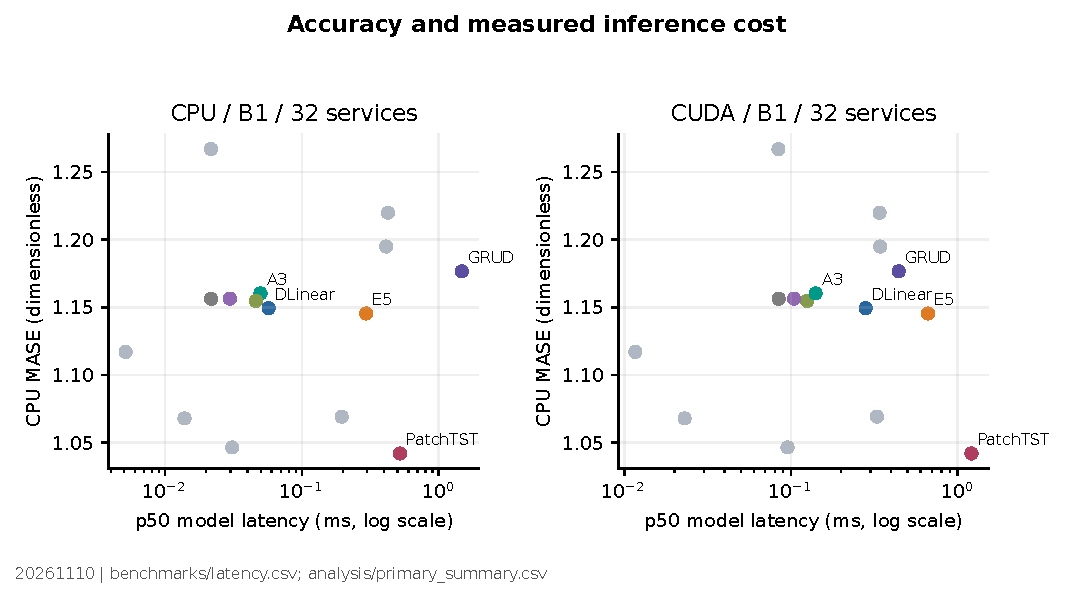
\includegraphics[width=0.79\textwidth]{figuras/13_latency.pdf}
\caption{CPU-resource MASE versus measured p50 forward latency. B1 inputs reside on the measured device. The laptop was shared, and these points exclude collection, preprocessing and control.}\label{fig:latency}\end{figure*}

\begin{figure*}[!t]\centering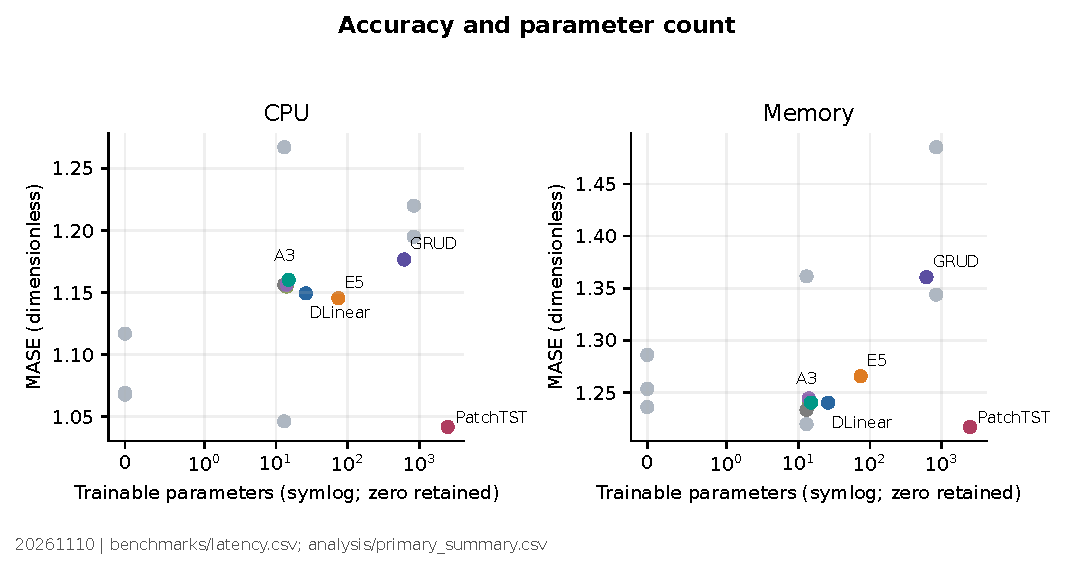
\includegraphics[width=0.79\textwidth]{figuras/14_parameters.pdf}
\caption{Error versus trainable count per resource. A symmetric-log axis retains zero-parameter references. Parameter counts exclude calibration and input state and therefore cannot substitute for measured memory or latency.}\label{fig:params}\end{figure*}

The resource monitor sampled one project-process RSS maximum of 1725.47 MiB; it did not capture a continuous peak. Whole-system RAM availability stayed above 10.87 GiB. Whole-system GPU memory in use reached 3536 MiB and the maximum recorded GPU temperature was $75^\circ$C; neither total can be attributed solely to our process. The CPU sensor reached $92^\circ$C and the study guard recorded one pause episode. The log retains seven failed GRU-D source attempts, 22 training OOM restart events and 94 inference batch-reduction events; the scheduled final fits and evaluations nonetheless have complete markers. Project energy was not measured.




